\documentclass{article}
\usepackage{graphicx}

\begin{document}
\title{ \normalsize \textsc{}
		\\ [2.0cm]
		\LARGE \textbf{\uppercase{Enhancing Camouflaged Object Segmentation in Limited Data Setting}
        }
		}
\date{\today}

\author{\textbf{Author} \\ 
		Vinitra Muralikrishnan}

{\let\newpage\relax\maketitle}
\tableofcontents
\newpage

\section{Style Transfer}

\subsection{About the algorithm}
It is an algorithm to transfer the styles of one image and modify the content of another image,
to match the style. This is done by formulating a loss function that matches the content and style of each
respective feature space of a deep network and then performing gradient descent on the pixels of the image itself.

\subsection{Loss function}
The loss function used to do this has 3 components: content loss, style loss and total variation loss. The content and style losses
will be used to penalized deviations from the content image and style image respectively.\\

\textbf{Content Loss:} The content loss will measure how much the feature map of the generated image differs from the feature map of the
source content image. The feature map in this case will belong to only one particular layer. Feature maps belong to the same layer will be
extracted from the 2 images and the distance between them will be calculated.\\
Let $F_{i,j}^{l}$ be the feature map from layer $l$ of the current image and $P_{i,j}^{l}$ be the feature map
from layer $l$ of the content source image.\\
$$L_c = w_c \times \sum_{i,j} (F_{i,j}^{l} - P_{i,j}^{l})^{2}$$

\textbf{Style Loss: } We compute the style loss using Gram matrix, which is the approximation to the covariance matrix.
This is done to get correlations between responses of each filter $F$ used above i.e we want the activation statistics
of our generated image to match the activation statistics of the style image. Given a feature map $F^l$ of shape
$(C_l, M_l)$, the gram matrix has shape $(C_l, C_l)$ and its elements are given by:\\
$$G_{i,j}^l = \sum_{k}F_{i,k}^l  F_{j,k}^l$$
Assuming $G^l$ is the Gram matrix of the feature map of the current image and $A^l$ is the gram matrix of the
feature map of the source style image and $w_l$ is a scalar weight term, then the style loss for the layer $l$
is simply the weighted Euclidean distance between 2 Gram matrices:\\
$$L_s^l = w_l \sum_{i,j} (G_{i,j}^l - A_{i,j}^l)^2$$
The final style loss from all the selected style layers would be:\\
$$L_s = \sum_{l \in L} L_s^l$$
\textbf{Total Variation Loss: } This component is a regularization term that penalizes sharp distortions that can
happen in the image when performing style transfer. This term encourages smoothness and is computed as the sum of the
squares of differences in the pixel values for all pairs of pixels that are next to each other (horizontally or vertically)
in all the channels:\\
$$L_{tv} = w_l \times \left( \sum_{c=1}^{3} \sum_{i=1}^{H-1} \sum_{j=1}^{W} (x_{i+1,j,c} - x_{i,j,c})^2 + \sum_{c=1}^{3} \sum_{i=1}^{H} \sum_{j=1}^{W-1} (x_{i,j+1,c} - x_{i,j,c})^2 \right)$$

\subsection{Examples}
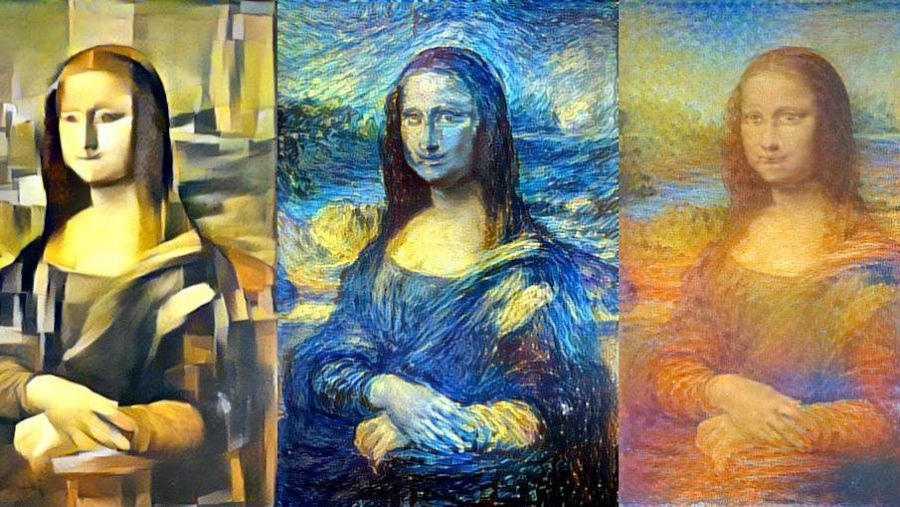
\includegraphics[width=5in]{./imgs/st-1.png}\\
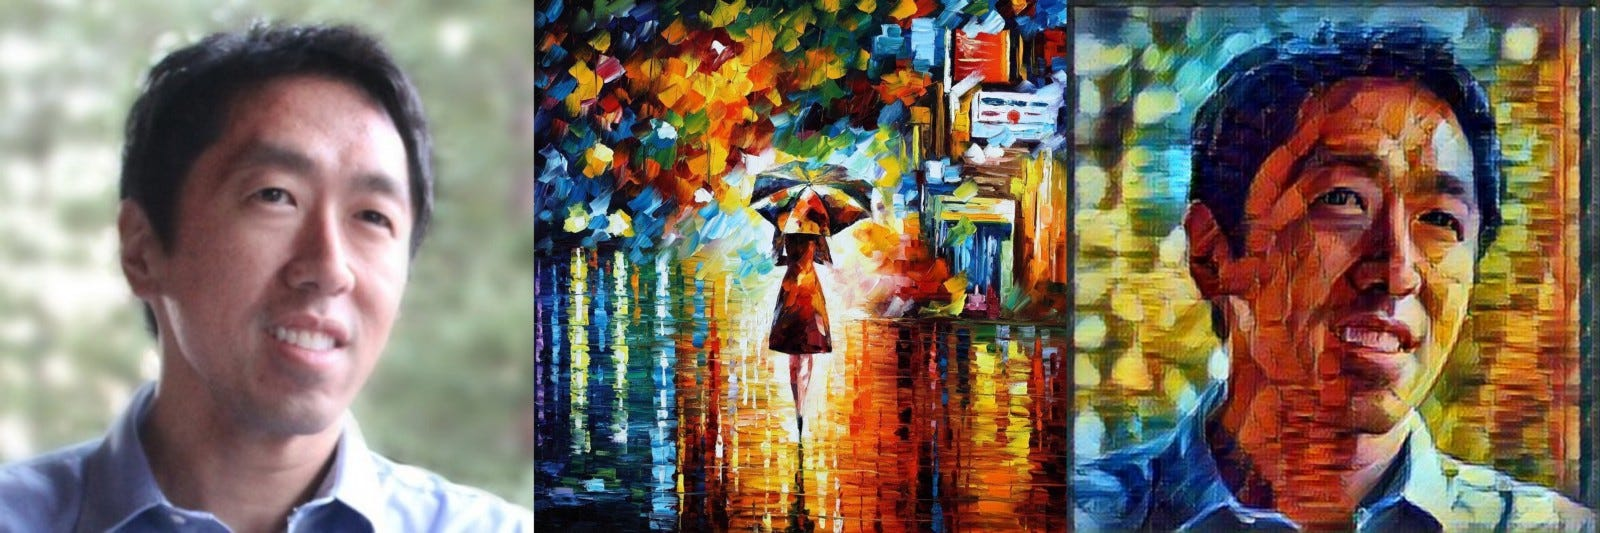
\includegraphics[width=5in]{./imgs/st-2.jpg}\\

\subsection{Questions and Answers}

\begin{enumerate}
	\item Why is only 1 content layer used but multiple style layers used in the algorithm?\\
	\textbf{Answer: } The answer lies in how neural networks capture information about the image. The content information 
	of images such as shapes, spatial features are high level features or the semantic meaning of the image. In CNNs, deeper layers
	capture the information that represent the overall content of the image. By using just 1 deeper layer, we can effectively capture the content
	as it contains enough semantic information to represent the overal structure of the image. To capture the style however,
	we need to capture textures, patterns and colors which is capture on different layers by different layers of CNNs. Shallow
	layers capture fine-grained details like edges and textures. Deeper layers, capture more abstract global patterns such as colors.
	By using both shallow and deeper layers in the style loss, we ensure that the transferred style captures both the low-level
	and high-level features. This multi-layer approach, provides a comprehensive representation of the style.
	\item Why use gram matrix for covariance approximation?
	It captures feature correlations such as textures. Additionally it is spatially independent, meaning that it ignores
	location of where the patterns occur but instead focuses on how strongly features correlate through image. This is important,
	because it allows the style transfer to happen on all locations in the generated image. Alternatively, this could possibly
	be hurdle in focusing style transfer on specific locations. Gram matrix is also simple and efficient to compute.
	\item Alternatives to Gram matrix?
	Covariance matrix might capture more nuanced relationships between feature maps because they consider the distribution
	of activations rather than just their dot product. This is one alternative to Gram matrix. Higher order statistics,
	while more more computationally expensive, captures more complex patterns in the distribution of activations across feature maps.
	Another alterantive is moment matching i.e matching moments of feature map activations like mean and variance. Moment matching focuses
	on normalizing feature statistics to align the style, particularly useful in methods like Adaptive Instance Normalization (AdaIN). Feature map
	histogram matching is also another alternative. But it captures only some aspects of style because it directly compares distribution
	of individual features, without computing correlations.
\end{enumerate}
\subsection{Ideas}
The idea is to replace gram matrix with a spatially dependent  metric to capture styles in local regions
instead of getting a global representation of styles. This might help constrain style transfer in specific regions
such as capturing styles of sky and transfer it only on the sky. The metrics that can be looked into are:\\
\begin{itemize}
	\item Deep Feature Correlation Matching: Captures local spatial correlations between features.
	\item Patch-Based Methods (Style Swap): Transfers patches of style based on local regions of the image, retaining spatial consistency.
	\item MRF Matching: Matches style patches based on spatial arrangements and local neighborhoods.
	\item Wasserstein Distance (Optimal Transport): Aligns feature distributions while considering the spatial arrangement.
	\item Histogram Matching with Spatial Constraints: Aligns feature histograms while enforcing spatial coherence.
	\item Texture-Synthesis Methods with Spatial Regularization: Synthesizes textures while preserving spatial relationships.
\end{itemize}
\clearpage
\section{SINet}
The SINet model is inspired by the human vision system and how it tackles camouflaged object segmentation. It is an architectural
framework that can be integrated with any model backbone such as Resnet or VGG.

\subsection{About the Architecture}
It is composed of 2 main modules - Search Module and Identification Module:\\
\textbf{Search module: } It leverages a series of Receptive Field blocks that mimics the human visual
system' strcture. These RF blocks help to highlight regions in the visual field at different scales and capture details
that help identify where a camouflaged object might be. This component comprises of several branches that capture details
at different scales and enhance the detection capabilities of the network by that.\\
\textbf{Identification module: } Following the detection of a potential camouflaged object by the SM, the IM precisely identifies
and segments the object. It utilizes a Partial Decoder Component that integrates with the multi-level features processed by the SM.
Partial Decoder Component refines the features from deeper layers of the network by emphasizing regions most likely to contain the
camouflaged objects. Unlike full decoders, PDC selectively refines only certain regions of interest to improve computational
efficiency. It then uses the information by decoder to further refine segmenation, specifically at teh boundaries of the object.
\section{Stable Diffusion}
Stable diffusion is a generative model designed to generate high-quality data. The generated data can also be conditioned
on some other input such as text. It leverages diffusion, where random noise is progressively added to a latent representation of an image
and then a NN is trained to reverse this process, gradually denoising image back to the clear representation. When conditioned on something,
such as text it uses cross attention mechanism to effectively combine teh text embedding with latent representation of the image.
This allows the model to incorporate meaning of the text into visual generation. The core architecture of the stable diffusion is
a UNet. During the training process, the images are corrupted with noise and then learning to reconstruct the original
image from denoising process. During training, it learns the mapping between text embeddings and corresponding images, so it can generate novel images
that match the text inputs.
\section{Segmentation}
\subsection{Evaluation metrics}
\begin{itemize}
	\item DICE: Measure the overlap between the prediction segmentation and the ground truth. Rnages from 0 to 1.
	\item IoU: Evaluates the similarity between the predicted segmentation and the ground truth by comparing their overlap
	\item P-Acc (Pixel Accuracy): Measures the proportion of correctly classified pixels in the segmentation result.
\end{itemize}
\section{Questions and Answers about Project}
\begin{enumerate}
	\item Why randomly sample 3k images from the generated 15k style transferred images?
	\textbf{Answer: } Since the number of generated iamges is much more than the original images available for training - about
	3k - sampling in every epoch helps maintain the balance between original and synthesized images while maintaining high
	diversity. The sampling will be done with the goal of covering all 15k samples in all epochs.
	\item Name the datasets used.
	\textbf{Answer: } COD10K, CAMO, CHAMELEON
\end{enumerate}
\end{document}



